\documentclass[12pt]{article}

% Idioma y codificación
\usepackage[spanish, es-tabla]{babel}       %es-tabla para que se titule "Tabla"
\usepackage[utf8]{inputenc}

% Márgenes
\usepackage[a4paper,top=3cm,bottom=2.5cm,left=3cm,right=3cm]{geometry}

% Comentarios de bloque
\usepackage{verbatim}

% Paquetes de links
\usepackage[hidelinks]{hyperref}    % Permite enlaces
\usepackage{url}                    % redirecciona a la web

% Más opciones para enumeraciones
\usepackage{enumitem}

% Personalizar la portada
\usepackage{titling}


% Paquetes de tablas
\usepackage{multirow}


%------------------------------------------------------------------------

%Paquetes de figuras
\usepackage{caption}
\usepackage{subcaption} % Figuras al lado de otras
\usepackage{float}      % Poner figuras en el sitio indicado H.


% Paquetes de imágenes
\usepackage{graphicx}       % Paquete para añadir imágenes
\usepackage{transparent}    % Para manejar la opacidad de las figuras

% Paquete para usar colores
\usepackage[dvipsnames]{xcolor}
\usepackage{pagecolor}      % Para cambiar el color de la página

% Habilita tamaños de fuente mayores
\usepackage{fix-cm}


%------------------------------------------------------------------------

% Paquetes de matemáticas
\usepackage{mathtools, amsfonts, amssymb, mathrsfs}
\usepackage[makeroom]{cancel}     % Simplificar tachando
\usepackage{polynom}    % Divisiones y Ruffini
\usepackage{units} % Para poner fracciones diagonales con \nicefrac

\usepackage{pgfplots}   %Representar funciones
\pgfplotsset{compat=1.18}  % Versión 1.18

\usepackage{tikz-cd}    % Para usar diagramas de composiciones
\usetikzlibrary{calc}   % Para usar cálculo de coordenadas en tikz

% Paquete para usar el símbolo de grados
\usepackage{gensymb}

%Definición de teoremas, etc.
\usepackage{amsthm}
%\swapnumbers   % Intercambia la posición del texto y de la numeración

\theoremstyle{plain}

\makeatletter
\@ifclassloaded{article}{
  \newtheorem{teo}{Teorema}[section]
}{
  \theoremstyle{definition}
  \newtheorem{teo}{Teorema}[chapter]  % Se resetea en cada chapter
}
\makeatother

\theoremstyle{definition}
\newtheorem{coro}{Corolario}[teo]           % Se resetea en cada teorema
\newtheorem{prop}[teo]{Proposición}         % Usa el mismo contador que teorema
\newtheorem{lema}[teo]{Lema}                % Usa el mismo contador que teorema

\theoremstyle{remark}
\newtheorem*{observacion}{Observación}

\theoremstyle{definition}

\makeatletter
\@ifclassloaded{article}{
  \newtheorem{definicion}{Definición} [section]     % Se resetea en cada chapter
}{
  \newtheorem{definicion}{Definición} [chapter]     % Se resetea en cada chapter
}
\makeatother

\newtheorem*{notacion}{Notación}
\newtheorem*{ejemplo}{Ejemplo}
\newtheorem*{ejercicio*}{Ejercicio}             % No numerado
\newtheorem{ejercicio}{Ejercicio} [section]     % Se resetea en cada section


% Modificar el formato de la numeración del teorema "ejercicio"
\renewcommand{\theejercicio}{%
  \ifnum\value{section}=0 % Si no se ha iniciado ninguna sección
    \arabic{ejercicio}% Solo mostrar el número de ejercicio
  \else
    \thesection.\arabic{ejercicio}% Mostrar número de sección y número de ejercicio
  \fi
}


\renewcommand\qedsymbol{\small{$\blacksquare$}}         % Cambiar símbolo QED
%------------------------------------------------------------------------

% Paquetes para encabezados
\usepackage{fancyhdr}
\pagestyle{fancy}
\fancyhf{}

\newcommand{\helv}{ % Modificación tamaño de letra
\fontfamily{}\fontsize{12}{12}\selectfont}
\setlength{\headheight}{15pt} % Amplía el tamaño del índice


%\usepackage{lastpage}   % Referenciar última pag   \pageref{LastPage}
\fancyfoot[C]{\thepage}

%------------------------------------------------------------------------

% Conseguir que no ponga "Capítulo 1". Sino solo "1."
\makeatletter
\@ifclassloaded{book}{
  \renewcommand{\chaptermark}[1]{\markboth{\thechapter.\ #1}{}} % En el encabezado
    
  \renewcommand{\@makechapterhead}[1]{%
  \vspace*{50\p@}%
  {\parindent \z@ \raggedright \normalfont
    \ifnum \c@secnumdepth >\m@ne
      \huge\bfseries \thechapter.\hspace{1em}\ignorespaces
    \fi
    \interlinepenalty\@M
    \Huge \bfseries #1\par\nobreak
    \vskip 40\p@
  }}
}
\makeatother

%------------------------------------------------------------------------
% Paquetes de cógido
\usepackage{minted}
\renewcommand\listingscaption{Código fuente}

\usepackage{fancyvrb}
% Personaliza el tamaño de los números de línea
\renewcommand{\theFancyVerbLine}{\small\arabic{FancyVerbLine}}

% Estilo para C++
\newminted{cpp}{
    frame=lines,
    framesep=2mm,
    baselinestretch=1.2,
    linenos,
    escapeinside=||
}


\usepackage{listings} % Para incluir código desde un archivo

\renewcommand\lstlistingname{Código Fuente}
\renewcommand\lstlistlistingname{Índice de Códigos Fuente}

% Definir colores
\definecolor{vscodepurple}{rgb}{0.5,0,0.5}
\definecolor{vscodeblue}{rgb}{0,0,0.8}
\definecolor{vscodegreen}{rgb}{0,0.5,0}
\definecolor{vscodegray}{rgb}{0.5,0.5,0.5}
\definecolor{vscodebackground}{rgb}{0.97,0.97,0.97}
\definecolor{vscodelightgray}{rgb}{0.9,0.9,0.9}

% Configuración para el estilo de C similar a VSCode
\lstdefinestyle{vscode_C}{
  backgroundcolor=\color{vscodebackground},
  commentstyle=\color{vscodegreen},
  keywordstyle=\color{vscodeblue},
  numberstyle=\tiny\color{vscodegray},
  stringstyle=\color{vscodepurple},
  basicstyle=\scriptsize\ttfamily,
  breakatwhitespace=false,
  breaklines=true,
  captionpos=b,
  keepspaces=true,
  numbers=left,
  numbersep=5pt,
  showspaces=false,
  showstringspaces=false,
  showtabs=false,
  tabsize=2,
  frame=tb,
  framerule=0pt,
  aboveskip=10pt,
  belowskip=10pt,
  xleftmargin=10pt,
  xrightmargin=10pt,
  framexleftmargin=10pt,
  framexrightmargin=10pt,
  framesep=0pt,
  rulecolor=\color{vscodelightgray},
  backgroundcolor=\color{vscodebackground},
}

%------------------------------------------------------------------------

% Comandos definidos
\newcommand{\bb}[1]{\mathbb{#1}}
\newcommand{\cc}[1]{\mathcal{#1}}

% I prefer the slanted \leq
\let\oldleq\leq % save them in case they're every wanted
\let\oldgeq\geq
\renewcommand{\leq}{\leqslant}
\renewcommand{\geq}{\geqslant}

% Si y solo si
\newcommand{\sii}{\iff}

% Letras griegas
\newcommand{\eps}{\epsilon}
\newcommand{\veps}{\varepsilon}
\newcommand{\lm}{\lambda}

\newcommand{\ol}{\overline}
\newcommand{\ul}{\underline}
\newcommand{\wt}{\widetilde}
\newcommand{\wh}{\widehat}

\let\oldvec\vec
\renewcommand{\vec}{\overrightarrow}

% Derivadas parciales
\newcommand{\del}[2]{\frac{\partial #1}{\partial #2}}
\newcommand{\Del}[3]{\frac{\partial^{#1} #2}{\partial^{#1} #3}}
\newcommand{\deld}[2]{\dfrac{\partial #1}{\partial #2}}
\newcommand{\Deld}[3]{\dfrac{\partial^{#1} #2}{\partial^{#1} #3}}


\newcommand{\AstIg}{\stackrel{(\ast)}{=}}
\newcommand{\Hop}{\stackrel{L'H\hat{o}pital}{=}}

\newcommand{\red}[1]{{\color{red}#1}} % Para integrales, destacar los cambios.

% Método de integración
\newcommand{\MetInt}[2]{
    \left[\begin{array}{c}
        #1 \\ #2
    \end{array}\right]
}

% Declarar aplicaciones
% 1. Nombre aplicación
% 2. Dominio
% 3. Codominio
% 4. Variable
% 5. Imagen de la variable
\newcommand{\Func}[5]{
    \begin{equation*}
        \begin{array}{rrll}
            #1:& #2 & \longrightarrow & #3\\
               & #4 & \longmapsto & #5
        \end{array}
    \end{equation*}
}

%------------------------------------------------------------------------
\setlength{\parindent}{0pt} % quitar la sangría

\setlist[itemize, 1]{label=\textbullet \textbf{)}}  % Cambiar las viñetas a círculos

\def\endsquare{%
  \begin{flushright}
      \small{$\blacksquare$}
  \end{flushright}
}

\newcommand{\apuntar}[1]{%
  \hyperlink{#1}{\textbf{(#1)}}%p
}

\newcommand{\objetivo}[1]{%
  \textbf{(\hypertarget{#1}{#1})}
}


\usepackage{xkeyval} % Para el paso de argumentos

\usepackage{graphicx}

% Definir la carpeta de las imágenes
\graphicspath{{../_assets}{../../_assets}{../../../_assets}}

% Definir el comando \portada
\makeatletter
\define@key{portada}{titulo}{\def\titulo{#1}}
\define@key{portada}{subtitulo}{\def\subtitulo{#1}}
\define@key{portada}{autor}{\def\autor{#1}}
\define@key{portada}{año}{\def\año{#1}}
\define@key{portada}{color página}{\def\colorpagina{#1}}
\define@key{portada}{imagen}{\def\imagen{#1}}

\newcommand*{\portada}[1][]{%
  % Encabezado
  \fancyhead[L]{\helv \titulo}
  \fancyhead[R]{\helv \nouppercase{\leftmark}}

    % Definimos las claves y sus valores por defecto
  \setkeys{portada}{%
    titulo=Sin Título,%
    subtitulo=Sin Subtítulo,%
    autor=Autor Desconocido,%
    año=Sin Año,%
    color página=white,%
    imagen=Logo-UGR-Black.png, #1}%
    \begin{titlepage}
        \centering
        \pagecolor{\colorpagina} % Cambia el color de fondo de la portada
        {\includegraphics[width=0.2\textwidth]{\imagen}\par}
        \vspace{1cm}
        {\bfseries\LARGE Universidad de Granada \par}
        \vspace{1cm}
        {\scshape\Large Doble Grado en Ingeniería Informática y Matemáticas \par}
        \vspace{3cm}
        {\scshape\Huge \titulo \par}
        \vspace{3cm}
        {\itshape\Large \subtitulo \par}
        \vfill
        {\Large Autor: \par}
        {\Large \autor \par}
        \vfill
        {\Large \año \par}
    \end{titlepage}%
    \pagecolor{white}
}

\begin{document}
    \portada[%
        titulo=Sistemas Concurrentes y Distribuidos,
        subtitulo=Seminario 1,
        autor=Jesús Muñoz Velasco,
        año=Curso 2024-2025,
        imagen=../../../../documents/_assets/Logo-UGR-Black.png]
        
    % \thispagestyle{empty}
    % \tableofcontents
    % \newpage

    \section{Seminario 1. Actividad propuesta.}
    
    Como se puede observar en el archivo adjuntado se ha optado por la ditribución de trabajo a las hebras de forma cíclica (ya que empíricamente ofrecía los mejores resultados) su implementación en código ha sido la siguiente: 

    \begin{minted}{cpp}
    double funcion_hebra( long i )
    {
        double suma = 0.0 ;

        // Cíclico
        for(int j=i; j<m; j+=n) {
            suma += f((j+0.5)/m );
        }

        return suma;
    }
    \end{minted}

    Tras compilar y ejecutar el programa obtenemos la siguiente salida:\\

    \begin{center}
        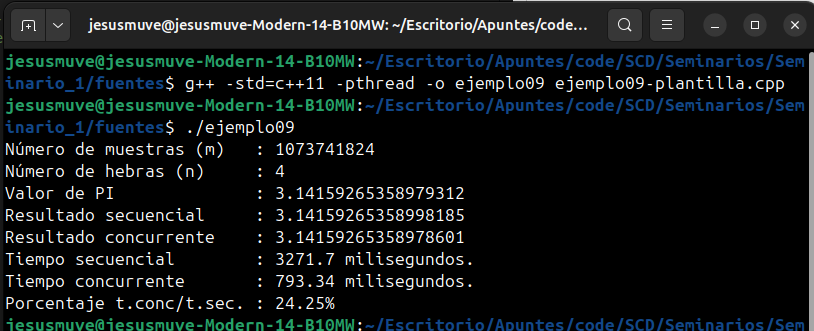
\includegraphics[width=15cm]{./salida_ejecucion.png}
    \end{center}

    Además, monitorizando los recursos del sistema (en concreto la CPU) podemos observar un pico general en 4 hebras al ejecutar el programa:

    \begin{center}
        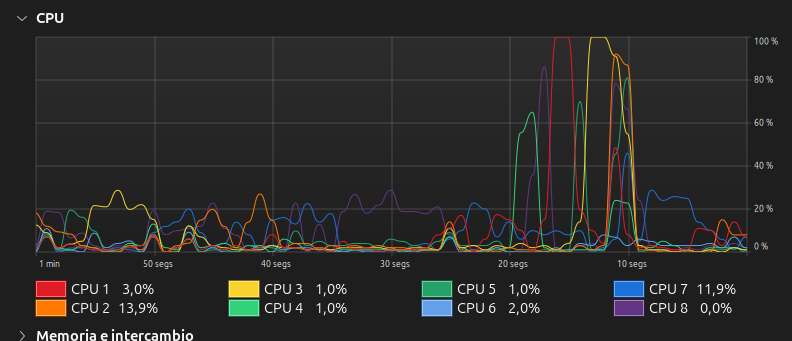
\includegraphics[width=15cm]{./recursos.png}
    \end{center}

    Además, en el código se han dejado 2 resoluciones más comentadas en el código: la repartición por bloques contiguos (vista en clase) y esta última pero reduciendo el número de divisiones (ya que es la operación más costosa). Sin embargo, por la precisión de mi ordenador no he podido obtener un resultado válido con este último método ya que aproxima la variable $paso=1/m$ a 0, no avanzando en el bucle y llegando a una condición de error (bucle infinito). Sin embargo, con un ordenador con una precisión mayor en la representación de números de coma flotante, esta debería ser la opción mejor.\\

    Voy a explicar de forma razonada la obtención de este código. En primer lugar, el código para bloques contiguos es el siguiente: 
    \begin{minted}{cpp}
    for(int j=(i*(m/n)); j<((i+1)*(m/n)); j++){ 
        suma += f( (j+0.5)/m );
    }
    \end{minted}

    El código ``mejorado'' es el siguiente:

    \begin{minted}{cpp}
    const long double medio=0.5/m;
    const long double paso=1/m;

    for(long double j=(i/n); j<((i+1)/n); j+=paso){ 
        suma += f( j+medio );
    }
    \end{minted}

    Como se puede ver se ha sustituido en primer lugar $j$ por $\frac{j}{m}$ obteniendo de la asignación inicial
    \begin{gather*}
        \frac{j}{m}=\frac{i*(m/n)}{m}=(i/n)
    \end{gather*}
    y de la condición.
    \begin{gather*}
        \frac{j}{m}<\frac{((i+1)*(m/n))}{m} = ((i+1)/n)
    \end{gather*}
    Además en el paso se deberá dividir también por $m$, siendo este valor constante y pudiendo ser calculado una sola vez (valor de la variable $paso$).\\

    En la ejecución de $f$ se han hecho los cambios pertinentes. Si llamamos a la $j$ actual $j'$ y a la anterior $j$ la dejamos como $j$ (siendo $j'=\frac{j}{m}$), podemos escribir $j=m*j'$, y sustituyendo esto en la línea de la ejecución de $f$ obtenemos
    \begin{gather*}
        f((j+0.5)/m) = f((m*j'+0.5)/m) = f(((m*j')/m) + (0.5/m)) = f(j'+ (0.5/m))
    \end{gather*}
    De esta forma podemos eliminar la división por $m$ en cada iteración definiendo la variable $medio$ con el valor $0.5/m$ que es constante. Con estos cambios habríamos reducido en cada iteración 2 productos (de la definición del bucle) y 1 división (de la ejecución de $f$). Sabiendo que $m$ que es el número de iteraciones es muy elevado esto supondría una gran mejora en la eficiencia y en la concurrencia. Esta misma solución se podría aplicar sobre la distribución cíclica pero obtendríamos el mismo problema con la precisión.

\end{document}